\documentclass[12pt]{../../notes}
\usepackage{silence}
\WarningFilter{latex}{Reference}
\graphicspath{{../../img/}}

\begin{document}
\paragraph{Интегральные неравенства}

\begin{stat}[Интегральное неравенство Йенсена]\label{stat:intjensen}
  Пусть $f \in C(I)$, где $I$~---промежуток; $f \convex I,\; \varphi \in C(I), \varphi \geqslant 0$.
  Тогда:
  \[
    f\left( \frac{\int_a^b x \varphi(x) \mathrm{d}x}{\int_a^b \varphi(x) \mathrm{d}x} \right) 
    \leqslant
    \frac{\int_a^b f(x) \varphi(x) \mathrm{d}x}{\int_a^b \varphi(x) \mathrm{d}x}
  \]
\end{stat}
\begin{ittproof}
  Заменим интегралы суммами Римана со следующими условиями:
  \[
    \tau = \left\{ a + \frac{b - a}{n} \right\},\; \xi_i = x_i\;\text{(левые прямоугольники)}
  \]
  Тогда \begin{align*}
    \sigma_1 = \sum_i \varphi(x_i)\Delta x_i = \frac{b - a}{n}\cdot\sum_{i=0}^{n-1}\varphi(x_i) 
    \xrightarrow[n\to\infty]{} \int_a^b \varphi(x)\mathrm{d}x = I_1 \\
    \sigma_2 = \sum_i x_i \varphi(x_i)\Delta x_i = \frac{b-a}{n}\cdot\sum_{i=0}^{n-1}x_i\varphi(x_i) 
    \xrightarrow[n\to\infty]{} \int_a^b x\varphi(x)\mathrm{d}x = I_2 \\
    \sigma_3 = \sum_i f(x_i)\varphi(x_i)\Delta x_i = 
    \frac{b-a}{n}\cdot\sum_{i=0}^{n-1}f(x_i)\varphi(x_i) \xrightarrow[n\to\infty]{} 
    \int_a^b f(x)\varphi(x)\mathrm{d}x = I_3 \\
  \end{align*}
  Пусть $\lambda_i = \frac{\varphi(x_i)}{\sum_i\varphi(x_i)} \geqslant 0$.
  Тогда из оригинальной теоремы Йенсена (\ref{thrm:jensen}) и Римана
  \[
    f\left( \sum_i \lambda_i x_i \right) \leqslant \sum_i \lambda_i f(x_i) \Leftrightarrow
    f\left( {\sigma_2\over \sigma_1} \right) \leqslant {\sigma_3\over\sigma_1}
    \xrightarrow[n\to\infty]{} f\left( {I_2\over I_1} \right) \leqslant {I_3\over I_1}
  \]\nopagebreak%
\end{ittproof}

\begin{stat}[Интегральное неравенство Гёльдера]\label{stat:intgeld}
  Пусть $\varphi,\psi \in C(I)$, где $I$~---промежуток, $\varphi,\psi \underset{I}{\geqslant} 0$ 
  (иначе степень не определена);
  $p,q > 1$, $\frac{1}{p} + \frac{1}{q} = 1$.
  Тогда:
  \begin{equation*}
    \int_a^b \varphi \psi \leqslant 
      \left( \int_a^b \varphi^p \right)^\frac{1}{q} \cdot \left( \int_a^b \psi^q \right)^\frac{1}{p} 
  \end{equation*}
\end{stat}

\paragraph{Формула Валлиса}
% XXX : ``правильная'' буква `d' будет теперь использоваться реально там где непонятно, а не где попало , она в интегралах выглядит некрасиво(..
\begin{lem}
  \[
    \forall n\in \N,\; n > 0 \; \int_0^{\lfrac{\pi}{2}} \sin^n\!x \,dx = \int_0^{\lfrac{\pi}{2}} \cos^n\!x \,dx 
    = \left\{ 
      \begin{array}{lll}
        \frac{(n-1)!!}{n!!}                     & , & n = 2k + 1 \\[0.3em]
        \frac{(n-1)!!}{n!!}\cdot \frac{\pi}{2}  & , & n = 2k
      \end{array}
      \right.(k \in \Z)
  \]
\end{lem}
\begin{itlproof}
  Если поинтегрировать по частям, получится соотношение:
  \[
    I_n = \frac{n-1}{n} I_{n-2}
  \]
  Всё сводится к двум ``отправным точкам''
  \[
    \begin{split}
      I_0 = \int_0^{\lfrac{\pi}{2}} 1 = \frac{\pi}{2} & \\
      I_1 = \int_0^{\lfrac{\pi}{2}} \sin x = 1 & \\
    \end{split}
  \]
  Отсюда очевидным образом получаются оба ответа
\end{itlproof}
\begin{thrm}[Формула Валлиса]\label{thrm:wallisf}
  \[
    \lim_{n\to\infty} \frac{\big( (2n)!! \big)^2}{(2n-1)!! (2n+1)!!} = \frac{\pi}{2}
  \]
\end{thrm}

\paragraph{Интегральная форма остаточного члена формулы Тейлора}
{ \thrm\label{thrm:intaylresidue} Пусть $f : I\to\R,\; f\in C^{n+1}(I),\; a\in I$. 
Тогда:
\begin{align*}
  f(x) &= T_n(x) + R_n(x), \\
  &\text{ где } T_n(x) = \sum_{k=0}^n\,\alpha_k(x-a)^k,  \\ 
  &R_n(x) = {1\over n!}\int_a^x f^{(n+1)}(t)(x-t)^{n}\,{\rm d}x ,\\
  &\alpha_k = {f^{(k)}(a) \over k!} 
\end{align*}
}
\paragraph{Аддитивные функции промежутка}
\begin{defn}\label{defn:addfunc}
  Пусть $\Delta$~--- промежуток. Тогда $\Phi(\Delta)$~--- аддитивная функция промежутка $\Delta$, если 
  \[
    \forall\,\alpha<\beta<\gamma \in \Delta \quad \Phi([\alpha;\gamma]) = \Phi([\alpha;\beta]) + \Phi([\beta;\gamma])
  \]
\end{defn}
\begin{exmp}
  $\Phi(\Delta) = |\Delta|$
\end{exmp}
{\defn\label{defn:avdens} $\frac{\Phi(\Delta)}{|\Delta|}$~--- средняя плотность аддитивной функции}

\begin{defn}\label{defn:pointdens} 
  Пусть $\Delta=[\alpha,\beta]$, $x \in \Delta$
  \[
    \lim_{\alpha,\beta \to x}\frac{\Phi(\Delta)}{|\Delta|} = \rho(x)
  \]
  $\rho(x)$~--- плотность аддитивной функции в точке.
\end{defn}

\begin{stat}
  Пусть $I = [A;B],\; x \in I$, $\Phi$~--- аддитивная функция на $I$, $\Delta \subset I$, $\Delta=[\alpha,\beta]$.
  Тогда если ввести такую функцию: $F(x) := \Phi([A,x])$, то $\Phi(\Delta) = F(\beta)-F(\alpha)$.
\end{stat}
{\lem\label{lem:densderiv} Если $\rho(x)$ существует, то $\rho(x) = F'(x)$}
\begin{lem}\label{lem:addintdens}
  Пусть $\Phi$~--- аддитивна на $I$, $\exists\, \rho \in C(I)$ , $\Delta = [\alpha,\beta]\in I$. Тогда
  \[
    \Phi(\Delta) = \int_\alpha^\beta \rho(x) dx
  \]
\end{lem}
\begin{exmp}
  Площадь криволинейной трапеции.
  \[
    S = \int_a^b f(x) dx
  \]
\end{exmp}

\paragraph{Тесты на плотность}

\begin{stat}\label{stat:denstest1}
  Пусть $\Phi$~--- аддитивная функция промежутка $\Delta \subset I$, 
  $f\in C(I)$, $m(\Delta), M(\Delta)$~--- ещё 2 функции от переменного промежутка $\Delta$. Если при этом:
  \begin{enumerate}
    \item $\forall\, \Delta \subset I \quad m(\Delta) \leqslant \frac{\Phi(\Delta)}{|\Delta|} \leqslant M(\Delta)$
    \item $\forall\, \Delta \subset I, \; \forall\, x\in \Delta \quad m(\Delta) \leqslant f(x) \leqslant M(\Delta)$
    \item $|\Delta|\to 0$ $\Rightarrow$ $M(\Delta) - m(\Delta) \to 0$
  \end{enumerate}
  то $\rho(x) = f(x)$
\end{stat}

\begin{stat}\label{stat:denstest2}
  Пусть $\Phi$~--- аддитивная функция промежутка $\Delta \subset I$, $f\in C(I)$ и 
  \[
    \forall\, \Delta \subset I \left( \min_\Delta f \right) \cdot |\Delta| 
    \leqslant \Phi(\Delta) \leqslant \left( \max_\Delta f \right)\cdot |\Delta|
  \] Тогда $\rho(x) = f(x) $
\end{stat}
  
\begin{stat}\label{stat:denstest3}
  Пусть $\Phi$~--- аддитивная функция промежутка $\Delta \subset I$, $f,g\in C(I)$, $f,g \geqslant 0$ и
  \[
    \forall\, \Delta \subset I \left( \min_\Delta \right) \cdot \left( \min_\Delta g \right) \cdot |\Delta|
    \leqslant \Phi(\Delta) 
    \leqslant \left( \max_\Delta f \right) \cdot \left( \max_\Delta g \right) \cdot |\Delta|
  \] Тогда $\rho(x) = f(x) g(x) $
\end{stat}

\paragraph{Площадь криволинейного сектора}
\def\Sec#1#2{\ensuremath\operatorname{Sec}_{#1}^{\,#2}}
\begin{defn}\label{defn:sector} 
  Пусть $I = [\varphi_1; \varphi_2]$, $g \in C(I)$, $g \geqslant 0$, $\Delta = [\alpha;\beta] \subset I$.
  Тогда
  \[
    %                             v<- equal to `|', but better spacing
    \Sec\Delta g = \{(r;\varphi) \mid \varphi \in \Delta, 0 \leqslant r \leqslant g(\varphi)\}
  \]
\end{defn}
\begin{thrm}\label{thrm:secarea}
  \[
    S(\Sec\Delta g) = \frac{1}{2} \int_\Delta g^2(\varphi) d\varphi
  \]
\end{thrm}
\paragraph{Объём тела вращения}

\begin{defn}\label{defn:rotbody} 
  Пусть $I = [\varphi_1; \varphi_2]$, $g \in C(I)$, $g \geqslant 0$, $\Delta = [\alpha;\beta] \subset I$.
  Тогда
  \[
    %                             v<- equal to `|', but better spacing
    \mathrm{B}_\Delta = \{(x;y;z)\in \R^3 \mid x \in \Delta, y^2 + z^2 \leqslant g^2(x)\}
  \]
\end{defn} 
\begin{thrm}\label{thrm:rotbodyarea}
  \[
    \operatorname{Vol}(\mathrm{B}_\Delta) = \pi \int_\Delta g^2(x) d\varphi
  \]
\end{thrm}
\begin{thrm}[Обобщение \ref{thrm:rotbodyarea}]
  Пусть $V$~--- объём трёхмерного тела, $S(x)$~--- площадь сечения плоскостью $\perp$ $OX$. Тогда
  \[
    V = \int_a^b S(x) dx
  \]
\end{thrm}
\paragraph{Приложение интегралов к физике}

\begin{exmp}
  Статический момент плоской фигуры
  относительно оси.
  
  \medskip

  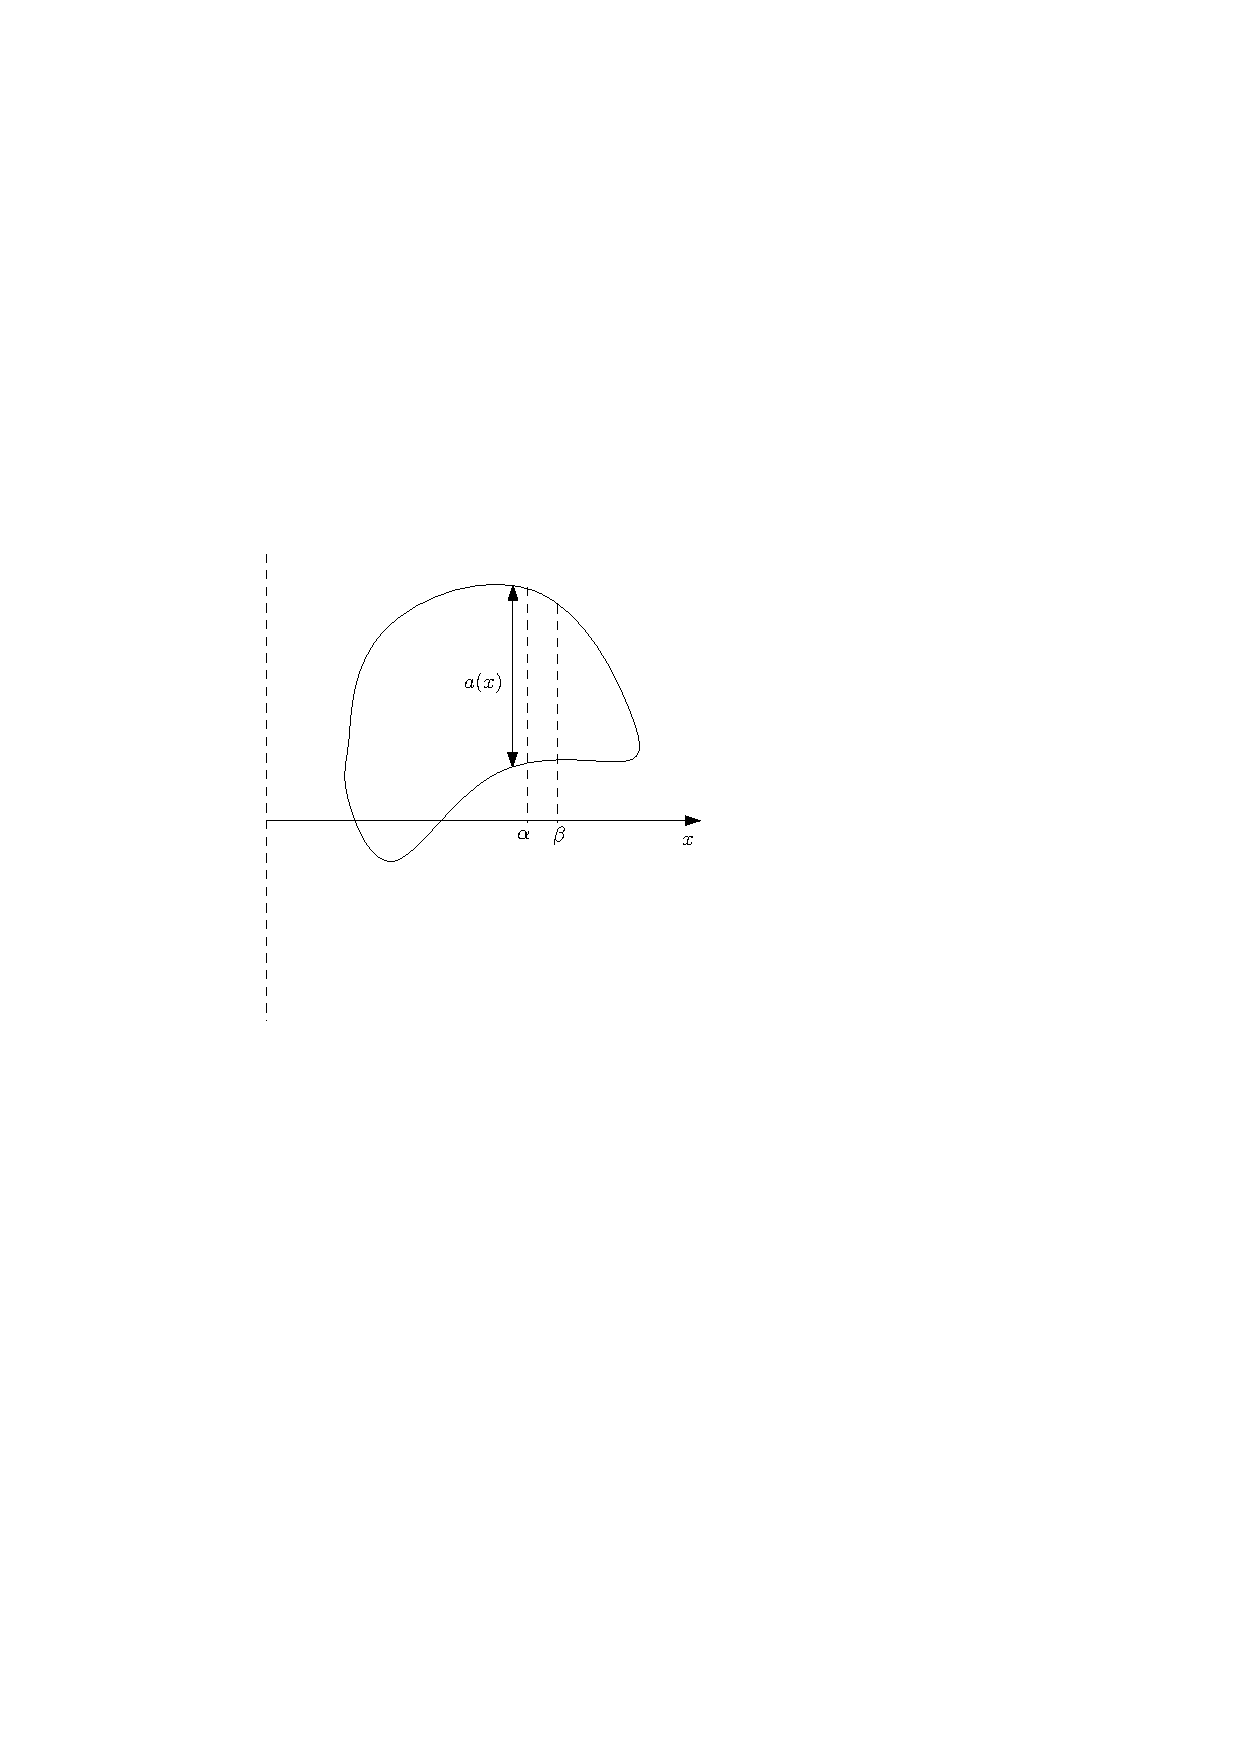
\includegraphics[scale=0.85]{moment}
  
  Докажем, что
  \[ 
    N = \int_{x_1}^{x_2} \sigma xa \left( x \right) \, d  x 
  \]
  где $a \left( x \right)$~--- длина ``сечения''
  фигуры, $\sigma$~--- поверхностная
  плотность
  
  Пусть $\Delta = [ \alpha, \beta ] \subset [ x_1, x_2 ]$~--- промежуток на оси $x$, 
  $\Phi ( \Delta )$~--- момент такой ``полоски''.
  
  Будем считать статический момент аддитивным по определению. Ещё мы умеем считать момент точки: он равен $m_i x_i$.
  Чтобы воспользоваться тестом~\ref{stat:denstest3} докажем, что (то, что они все положительные, очевидно)
  \[ 
    \left( \min_{\Delta} a \left( x \right) \right)  \left( \min_{\Delta} x
    \sigma \right)  \left| \Delta \right| \leqslant \Phi \left( \Delta
    \right) \leqslant \left( \max_{\Delta} a \left( x \right) \right)  \left(
    \max_{\Delta} x \sigma \right) \left| \Delta \right| 
   \]
  \begin{align*}
    & \left( \min_{\Delta} a \left( x \right) \right)  \left| \Delta
    \right| = \left| \Delta \right| a_{\min} = S_1 \text{~---вписанная площадь полоски}\\
    & \left( \max_{\Delta} a \left( x \right) \right)  \left| \Delta
    \right| = \left| \Delta \right| a_{\max} = S_2 \text{~---описанная площадь полоски}\\
    & \left( \min_{\Delta} x \right) = \alpha \\
    & \left(\max_{\Delta} x \right) = \beta 
  \end{align*}
  
  Тогда нижний предел~--- это если бы мы
  сгребли всю массу с $S_1$ и поместили в
  ближний к оси край и посчитали момент
  всего этого. Видно, что момент полоски на
  самом деле больше: и масса оценена снизу,
  и есть хотя бы одна точка с ненулевой
  массой дальше от оси чем $\alpha$.
  Аналогичные рассуждения применимы про
  оценку сверху.
  
  Все условия теста \ref{stat:denstest3} выполнены,
  значит
  \[ 
    N_{\Delta} = \Phi \left( \Delta \right) = \int_{\Delta} a(x) x \sigma \, d  x 
   \]
\end{exmp}

\begin{exmp}
  Работа, которую нужно затратить на
  возведение пирамиды.
  
  \medskip
  
  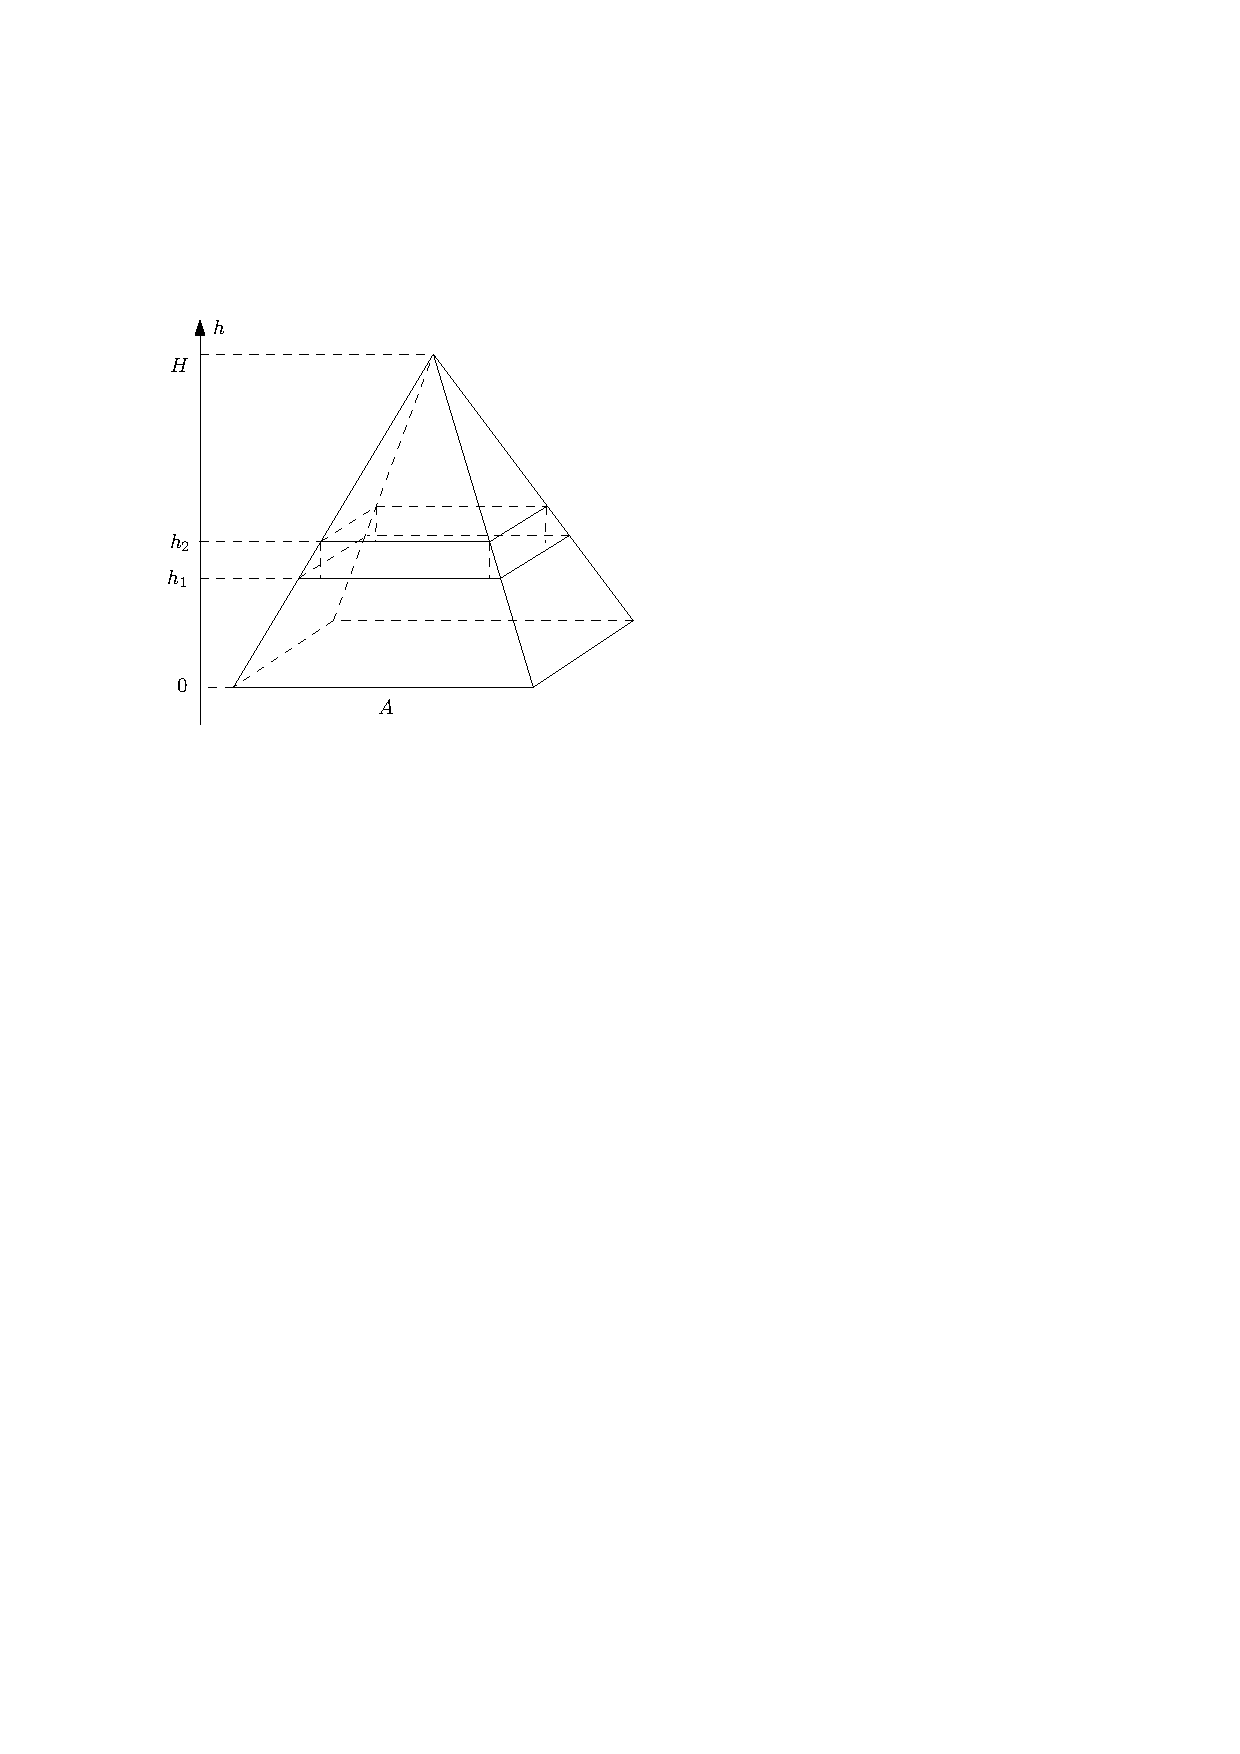
\includegraphics[scale=0.85]{pir}
  
  Пусть $\Delta = \left[ h_1, h_2 \right] \subset \left[ 0 ; H \right]$~--- промежуток на оси высот, 
  $\Phi \left(\Delta \right)$~--- работа которую нужно
  затратить чтобы поднять слой толщины $\left| \Delta \right|$ на нужную высоту, $a \left( h \right)$~---
  сторона пирамиды в зависимости от высоты (она правильная и с квадратом в  основании).
  
  Чтобы получить функцию плотности,
  посмотрим сначала, что происходит с
  блоком в форме параллелепипеда со
  стороной основания $a$. Если поднять его на
  высоту $h$ то работа, затрачена на это
  --- $mgh = \rho a \left( h \right)^2 hg$.
  
  Теперь, давайте докажем, что
  \[ 
    \Phi \left( \Delta \right) = \int_{\Delta} a \left( h \right)^2 hg \, d h 
  \]
  
  
  Будем пользоваться условием теста
  \ref{stat:denstest3}
  \[ \left( \min_{\Delta} a \left( x \right)^2 \right)  \left( \min_{\Delta}
     x \rho \right)  \left| \Delta \right| \leqslant \Phi \left( \Delta
    \right) \leqslant \left( \max_{\Delta} a \left( x \right)^2 \right) 
    \left( \max_{\Delta} x \rho \right) \left| \Delta \right| 
  \]
  
  
  Как видно, от предыдущего примера
  отличается только степенью при $a \left( x
  \right)$. Доказательство здесь почти такое
  же, разве что вместо площадей~--- объёмы.
  
  У нормальной пирамиды $a \left( h \right) = A \frac{H - h}{H}$. Тогда
  \[ 
    A = \int_0^H A^2  \left( 1 - \frac{h}{H} \right)^2 h \rho \, d \, x =
    \rho \frac{A^2}{H^2}  \left( \frac{H^4}{2} - \frac{2 H^4}{3} +
    \frac{H^4}{4} \right) = \frac{1}{12} \rho A^2 H^2 
  \]
  
\end{exmp}

\paragraph{Путь и кривая}
\begin{defn}\label{defn:path}
  Пусть $\gamma \colon [a;b] \to \R^2$, $\gamma$~--- непрерывна (в многомерном смысле). 
  Тогда $\gamma$~--- \emph{путь} на плоскости. Путь~--- отображение.
\end{defn}
\begin{defn}\label{defn:pathcarr}
  Множество $\Gamma = \gamma([a;b])$~--- носитель пути. $\gamma$ в таком случае называется \emph{параметризацией}
  $\Gamma$. 
\end{defn}

\begin{defn}\label{defn:simppath}
  Путь называется \emph{простым}, если отображение $\gamma$~--- биекция.
\end{defn}

\begin{defn}\label{defn:curve}
  Носитель простого пути называется \emph{кривой} \cite{zorich} в $\R^2$ (ну или в $\R^3$, путь туда был).
\end{defn}

\begin{rem*}
  Полезно заметить, что у одной и той же кривой есть много параметризаций. 
\end{rem*}

\begin{exmp*}
  \begin{align*}
    \gamma_1 : 
    \begin{cases}
      x(t) = t \\
      y(t) = t
    \end{cases}, t \in (0;+\infty) & &
    \gamma_2 :
    \begin{cases}
      x(t) = e^{t^3-547} \\
      y(t) = e^{t^3-547} \\
    \end{cases}, t \in \R
  \end{align*}
\end{exmp*}

\begin{defn}\label{defn:curvelen}
  Пусть $\Gamma$~--- кривая, $\gamma\colon [a;b] \to \R^2$~--- её параметризация.

  \begin{tabular}[h]{ll}
    $\tau: a = t_0 < t_1 < \dotsb < t_n = b$ & разбиение отрезка $[a;b]$ \\
    $A_i = \gamma(t_i)$, $p(\tau) = A_1\dotso A_n$ & ломанная, вписанная кривую \\
    $\displaystyle \ell(p(\tau)) = \sum_{i=0}^{n-1} |A_iA_{i+1}|$ & длина ломанной
  \end{tabular}
  
  Тогда длина пути определяется так:\footnote{Длину кривой мы видимо считаем по определению равной длине пути}
  \[
    l(\gamma) := \sup_\tau \ell(p(\tau))
  \]
  При таком определении аддитивность вроде как очевидна ($\sup (\ell_1+\ell_2) = \sup \ell_1 + \sup \ell_2$).
\end{defn}

\paragraph{Вычисление длины гладкого пути}
\begin{thrm}
  Пусть $\Gamma$~--- кривая с гладкой параметризацией $\gamma \colon [a;b]\to R$, $\gamma(t) = (x(t),y(t))$,
  $\gamma \in C^1([a;b])$.
  Тогда длину пути можно найти так: 
  \[
    \ell = \int_a^b \sqrt{x'^2+y'^2} = \int_a^b |\gamma'| \quad \forall\,\gamma
  \]
\end{thrm}
\begin{ittproof}
  Пусть $[\alpha, \beta]=\Delta \subset [a;b]$, $\Phi(\Delta) = \ell(\gamma\big|_\Delta)$. К тому же, как заметили
  выше, $\Phi$~--- аддитивна. Докажем, что $\gamma'$~--- её плотность.

  Будем пытаться свести всё к тесту~\ref{stat:denstest1}. Пусть 
  \begin{align*}
    & m(\Delta) = \sqrt{\left( \min_\Delta |x'(t)| \right)^2 + \left( \min_\Delta |y'(t)| \right)^2}\\
    & M(\Delta) = \sqrt{\left( \max_\Delta |x'(t)| \right)^2 + \left( \max_\Delta |y'(t)| \right)^2}
  \end{align*}
  Условия теста:
  \begin{enumerate}
    \item $m(\Delta) \leqslant \dfrac{\ell(\Gamma_\Delta)}{|[\alpha;\beta]|} \leqslant M(\Delta)$ \\
      Посмотрим на кусочек кривой, который $\gamma(\Delta)$. Разобьём отрезок $[\alpha;\beta]$ 
      и приблизим кривую ломаной, как это делали в~\ref{defn:curvelen}. Тогда по теореме Лагранжа 
      длину звена ломаной можно записать так
      \begin{align*}
        & |A_i A_{i+1}| = \sqrt{|\Delta x_i|^2 + |\Delta y|^2}  = |\Delta t_i|\sqrt{(x'(\xi_1))^2 + (y'(\xi_2))^2}\\
        & |\Delta x_i| = |x'(\xi_1) \Delta t_i|, \; \xi_1 \in [t_i; t_{i+1}] \subset \Delta\\
        & |\Delta y_i| = |y'(\xi_2) \Delta t_i|, \; \xi_2 \in [t_i; t_{i+1}] \subset \Delta
      \end{align*}
      Отсюда понятно как ограничить длину звена 
      \[
        m(\Delta)|\Delta t_i| \leqslant |A_i A_{i+1}| \leqslant M(\Delta) |\Delta t_i|
      \]
      Сложим все такие неравенства:
      \[
        m(\Delta)|\Delta| \leqslant \ell(p) \leqslant M(\Delta) |\Delta|
      \]
      Перейдём к супремуму:
      \[
        m(\Delta) |\Delta| \leqslant \Phi(\Delta) \leqslant M(\Delta) |\Delta|
      \]
    \item очевидно из определения $m, M$
    \item из теоремы Вейерштрасса 
      \[
        \exists\, t^m , t_m \in \Delta \colon |x'(t_m)| = \min_\Delta |x'(t)|, |x'(t^m)| = \max_\Delta |x'(t)|
      \]
      Тогда при $\alpha,\beta \to t$ точки где достигаются экстремальные значения
      $t_m, t^m \to x$ и по непрерывности $x(t)$ $x(t_m),x(t^m) \to x(t)$.
      То же самое рассуждение и для $y(t)$ применимо. А тогда $|m(\Delta)-M(\Delta)|\to0$.
  \end{enumerate}
  Все условия выполнены, значит
  \[
    \Phi(\Delta) = \int_\Delta |\gamma'| \Rightarrow \ell(\gamma)  = \int_{a}^{b} |\gamma'(t)|\,dt
  \]
\end{ittproof}

\paragraph{Геометрический смысл обратных тригонометрических функций }
\def\arch{\ensuremath \operatorname{arch}}
\begin{figure}[t]
  \centering
  \begin{minipage}{0.48\linewidth}
    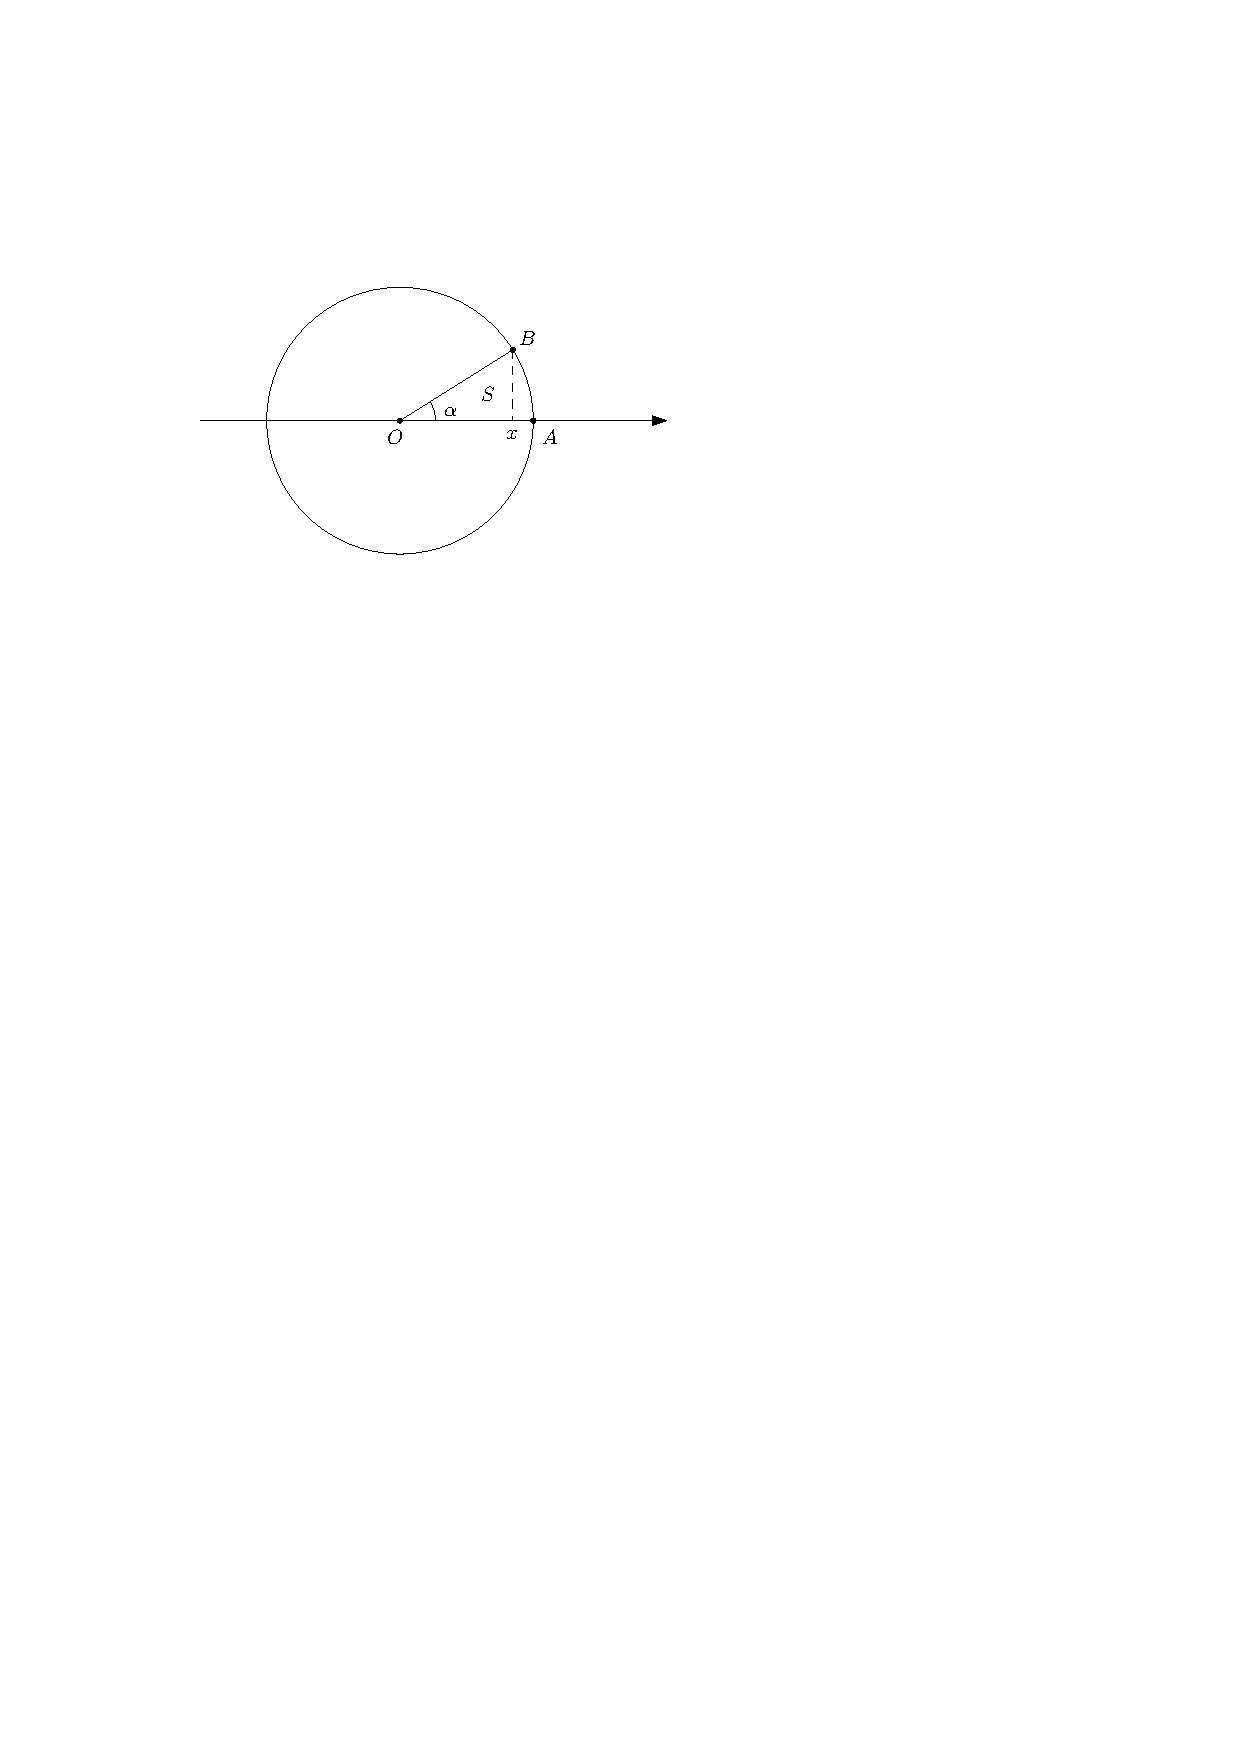
\includegraphics[scale=0.85]{acosgeomsense}~
  \end{minipage}
  \hfill
  \begin{minipage}{0.48\linewidth}
    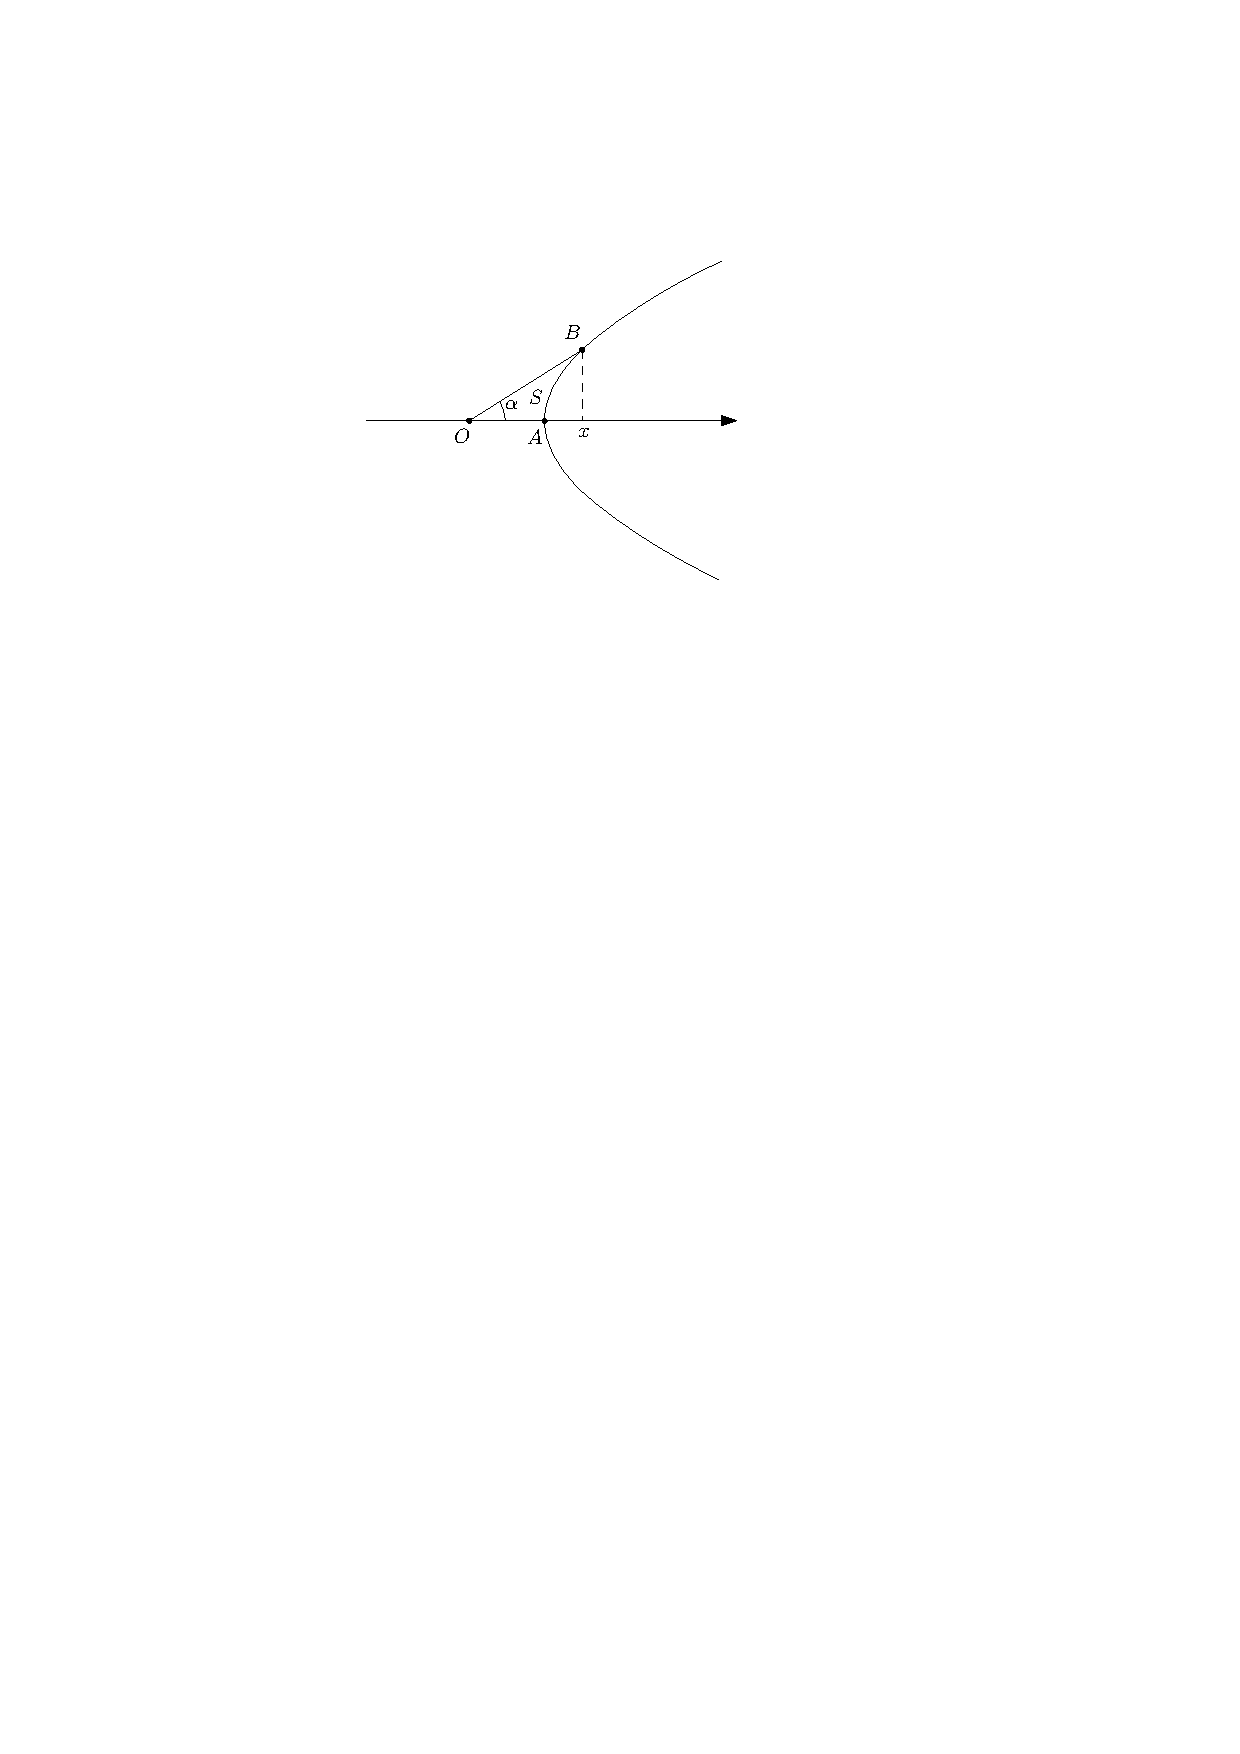
\includegraphics[scale=0.85]{achgeomsense}
  \end{minipage}
  \caption{Иллюстрация к геометрическому смыслу}
  \label{fig:acgeomsense}
\end{figure}
см. Рис.~\ref{fig:acgeomsense} 
\begin{align}
  &x = \cos t \Rightarrow t = \arccos x = \frac{1}{2}S_{AOB} \\
  &x = \ch t \Rightarrow t = \arch x = 2S_{AOB}
\end{align}
\end{document}
